\documentclass[14pt, aspectratio=169]{beamer}
\usepackage[utf8]{inputenc}
\usepackage[T2A]{fontenc}
\usepackage[russian]{babel}
\usepackage{listings}
\usepackage{xcolor}
\usepackage{amsmath}
\usepackage{amssymb}
\usepackage{graphicx}
\usepackage{tikz}
\usetikzlibrary{patterns}
\usepackage{adjustbox}

\definecolor{primary}{RGB}{41,128,185}
\definecolor{secondary}{RGB}{52,152,219}
\definecolor{accent}{RGB}{231,76,60}

\setbeamercolor{title}{fg=white, bg=primary}
\setbeamercolor{frametitle}{fg=white, bg=secondary}
\setbeamercolor{block title}{fg=white, bg=accent}

\setbeamerfont{frametitle}{size=\small}
\setbeamerfont{block title}{size=\footnotesize}

\setbeamertemplate{navigation symbols}{}
\setbeamertemplate{footline}{\hfill\insertframenumber/\inserttotalframenumber\hspace{1em}}

\lstset{
    language=C++,
    basicstyle=\ttfamily\tiny,
    keywordstyle=\color{blue},
    commentstyle=\color{green!60!black},
    stringstyle=\color{red},
    numbers=left,
    numberstyle=\tiny\color{gray},
    stepnumber=1,
    numbersep=2pt,
    backgroundcolor=\color{white},
    showspaces=false,
    showstringspaces=false,
    showtabs=false,
    frame=single,
    tabsize=2,
    captionpos=b,
    breaklines=true,
    breakatwhitespace=true
}

\title{Алгоритм проталкивания предпотока (Push-Relabel)}
\author{Антонов Кирилл \\ Б01-411}
\date{Курс «Алгоритмы и структуры данных»}

\begin{document}

\begin{frame}
\titlepage
\end{frame}

\begin{frame}{Мотивация: поиск максимального потока в больших сетях}
\scriptsize
\begin{block}{Проблема}
Задача о максимальном потоке заключается в том, чтобы найти наибольший объём жидкости (или данных), который можно передать из истока в сток с учётом пропускных способностей рёбер. \\
Классические алгоритмы (Форд-Фалкерсон, Диниц) на каждом шаге ищут увеличивающий путь от истока до стока. В больших графах (миллионы узлов) каждый такой поиск требует обхода значительной части графа, что приводит к высокому времени работы.
\end{block}

\begin{block}{Идея}
Можно отказаться от поиска полных путей и работать локально: проталкивать поток по одному ребру за раз, временно нарушая закон сохранения потока в узлах.
\end{block}

\begin{alertblock}{Вывод}
Для больших плотных графов требуется алгоритм без глобального поиска путей — таким является алгоритм проталкивания предпотока (push-relabel).
\end{alertblock}

\end{frame}

\begin{frame}{Постановка задачи о максимальном потоке}
\scriptsize
\begin{columns}[T]
\begin{column}{0.6\textwidth}
\begin{block}{Что дано}
Задан ориентированный граф $G = (V, E)$ с выделенными вершинами: истоком $s$ и стоком $t$. Каждому ребру $(u, v)$ приписана пропускная способность $c(u, v) \geq 0$ — максимальный объём потока, который может пройти по этому ребру.
\end{block}

\begin{block}{Что нужно найти}
Функцию $f: V \times V \to \mathbb{R}_{\geq 0}$, называемую \textbf{потоком}, такую что:
\begin{itemize}
\item $0 \leq f(u, v) \leq c(u, v)$ для всех $(u, v)$ — ограничение пропускной способности
\item $\sum_{v} f(u, v) = \sum_{v} f(v, u)$ для всех $u \notin \{s, t\}$ — закон сохранения потока (сколько втекло, столько и вытекло)
\end{itemize}
Цель: максимизировать суммарный поток, выходящий из истока:
\[
\text{maximize} \quad \sum_{v} f(s, v)
\]
\end{block}
\end{column}

\begin{column}{0.35\textwidth}
\begin{center}
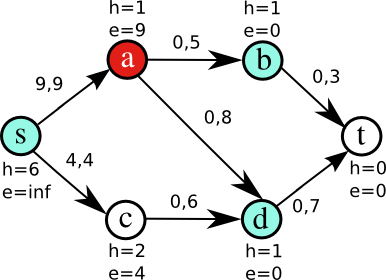
\includegraphics[width=\textwidth]{Flow_scale_1.png}
\small{Пример графа с пропускными способностями}
\end{center}
\end{column}
\end{columns}
\end{frame}

\begin{frame}{Ключевая идея: предпоток (preflow)}
\scriptsize
\begin{block}{Поток}
В классическом определении поток в промежуточных узлах должен сохраняться: сколько втекло, столько и вытекло. Это глобальное условие, которое алгоритмы вроде Диница поддерживают на каждом шаге.
\end{block}

\begin{block}{Предпоток}
Алгоритм проталкивания ослабляет это требование: в узлах может временно накапливаться избыток $e(u) \ge 0$, где
\[
e(u) = \sum_{v} f(v, u) - \sum_{v} f(u, v)
\]
Узлы с положительным избытком называются \textbf{активными}. Именно они обрабатываются алгоритмом.
\end{block}

\begin{block}{Зачем это нужно}
Ослабление условий позволяет работать локально: мы не ищем пути от истока до стока, а просто проталкиваем поток из активных узлов к соседям. Глобальный баланс восстановится сам собой в конце алгоритма, когда активных узлов не останется.
\end{block}

\begin{alertblock}{Важно}
Алгоритм начинает работу с предпотока (есть избытки) и заканчивает настоящим потоком (избытков нет).
\end{alertblock}
\end{frame}

\begin{frame}{Основные понятия: высота (height)}
\scriptsize
\begin{block}{Высота вершины $h(u)$}
\begin{itemize}
\item Искусственная «гравитация». В аналогии с водой и трубами: вода течёт только \textbf{вниз}
\item Целое неотрицательное число. Изначально: $h(s) = |V|$ (больше всех), $h(t) = 0$ (ниже всех), для остальных $h = 0$ % + пояснение
\item Высота может только увеличиваться (операция relabel)
\end{itemize}
\end{block}

\begin{block}{Правило течения}
Вода может быть протолкнута из $u$ в $v$ (операция push), только если:
\begin{itemize}
\item Остаточная пропускная способность $c_f(u, v) > 0$
\item $h(u) = h(v) + 1$ (течёт ровно на 1 уровень вниз)
\end{itemize}
\end{block}

\begin{block}{Как используются высоты}
\begin{itemize}
\item Направляют поток к стоку: сток имеет минимальную высоту 0, поэтому поток стремится вниз
\item Предотвращают зацикливание: высоты только растут, поэтому вода не может бесконечно циркулировать
\item Активный узел ($e(u) > 0$) либо проталкивает поток (если есть сосед на $h-1$), либо повышает свою высоту (relabel)
\end{itemize}
\end{block}
\end{frame}

\begin{frame}{Операции алгоритма}
\scriptsize

\begin{block}{Инициализация}
\begin{itemize}
\item $h(s) = |V|$ (самый высокий), $h(t) = 0$ (самый низкий), остальные также $h = 0$
\item Насыщаем все рёбра из истока: проталкиваем максимально возможный поток $c(s, v)$
\item У истока образуется отрицательный избыток (дефицит), у его соседей — положительный избыток
\end{itemize}
\end{block}

\begin{block}{Операция Push (проталкивание)}
\textbf{Условия:} узел $u$ имеет избыток ($e(u) > 0$), ребро $u \to v$ имеет остаточную пропускную способность ($c_f > 0$), и $h(u) = h(v) + 1$ (течёт ровно на 1 вниз) \\
\textbf{Действие:} пересылаем $\min(e(u), c_f(u, v))$ единиц потока из $u$ в $v$. После этого $u$ может перестать быть активным, а $v$ — стать активным.
\end{block}

\begin{block}{Операция Relabel (подъём)}
\textbf{Условия:} узел $u$ имеет избыток ($e(u) > 0$), но нет соседа, подходящего для push (все соседи с $c_f > 0$ имеют высоту $\ge h(u)$) \\
\textbf{Действие:} увеличиваем высоту $u$ до значения, чтобы появился сосед на 1 ниже: $h(u) = 1 + \min\{h(v) \mid c_f(u, v) > 0\}$. После подъёма становится возможен push.
\end{block}

\end{frame}

\begin{frame}{Корректность и завершимость}
\scriptsize

\begin{block}{Инварианты}
\begin{itemize}
\item \textbf{Направление потока:} push только при $h(u) = h(v) + 1$ (строго вниз)
\item \textbf{Монотонность высот:} $h(u)$ только увеличивается (relabel)
\item \textbf{Исток и сток:} $h(s) = |V|$, $h(t) = 0$ всегда
\end{itemize}
\end{block}

\begin{block}{Ограничение на число операций}
\begin{itemize}
\item Каждый relabel увеличивает $h(u)$, максимум $h(u) \le 2|V|$ → $O(|V|^2)$ релейблов
\item Насыщающий push уменьшает суммарный избыток
\item Ненасыщающий push переносит избыток ближе к стоку
\end{itemize}
\end{block}

\begin{block}{Итог}
Алгоритм всегда завершается, так как число операций ограничено. После завершения избытков нет — получен максимальный поток.
\end{block}

\end{frame}

\begin{frame}{Применение в реальных задачах}
\scriptsize
\begin{block}{Где используется максимальный поток}
\begin{itemize}
\item \textbf{Интернет-маршрутизация}: распределение трафика по каналам
\item \textbf{Логистика}: максимальный объём груза по сети дорог
\item \textbf{Сегментация изображений}: разрезание графа (Graph Cut)
\item \textbf{Распределение задач}: назначение работников на операции
\end{itemize}
\end{block}

\begin{block}{Почему выбирают push-relabel}
\begin{itemize}
\item Локальность работы → хорошая кэш-эффективность
\item Легко параллелится (можно толкать из нескольких узлов одновременно)
+ Один из самых быстрых на плотных графах
\end{itemize}
\end{block}

\end{frame}

\begin{frame}{Оценка времени работы}
\scriptsize

\begin{block}{Базовая версия (без эвристик)}
\[
O(V^2 \cdot E)
\]
Достигается за счёт того, что каждый relabel увеличивает высоту узла (не более $O(V)$ раз на узел), а каждый push может насытить ребро не более $O(V)$ раз.
\end{block}

\begin{block}{Улучшенные версии}
\begin{itemize}
\item \textbf{FIFO (очередь)}: $O(V^3)$ — обрабатывает активные узлы в порядке очереди
\item \textbf{Highest-Label + Gap эвристики (HLPP)}: $O(V^2 \sqrt{E})$ — выбирает узел с максимальной высотой, пропускает недостижимые высоты
\end{itemize}
\end{block}

\begin{block}{Число операций}
\begin{itemize}
\item Relabel: $O(V^2)$ (каждый узел может быть поднят не более $2V$ раз)
\item Push: $O(V^2 \cdot E)$ в базовой версии, меньше в HLPP
\end{itemize}
\end{block}

Подробные доказательства оценок приведены в литературе: \href{https://neerc.ifmo.ru/wiki/index.php?title=Метод_проталкивания_предпотока}{НИУ ИТМО: Алгоритм проталкивания предпотока}


\end{frame}

\begin{frame}{Сравнение алгоритмов поиска потока}
\scriptsize

\begin{block}{Теоретическая сложность}
\begin{adjustbox}{max width=\textwidth}
\begin{tabular}{|l|c|l|}
\hline
\textbf{Алгоритм} & \textbf{Сложность} & \textbf{Особенности} \\
\hline
Форд-Фалкерсон & $O(E \cdot f_{max})$ & Простой, но может работать очень долго при больших потоках \\
\hline
Диниц & $O(V^2 E)$ & Хорош на разреженных графах, использует BFS + DFS \\
\hline
Push-Relabel (базовый) & $O(V^2 E)$ & Работает локально, но без эвристик медленнее \\
\hline
Push-Relabel (HLPP) & $O(V^2 \sqrt{E})$ & С эвристиками Highest-Label и Gap — самый быстрый на плотных графах \\
\hline
\end{tabular}
\end{adjustbox}
\end{block}

\begin{block}{Ключевые различия}
\begin{itemize}
\item \textbf{Диниц} требует глобального поиска увеличивающих путей (BFS/DFS), что даёт преимущество на разреженных графах
\item \textbf{Push-Relabel} работает локально (только push/relabel), не ищет пути целиком — выигрывает на плотных графах, где путей слишком много
\item \textbf{HLPP-эвристики} (Highest-Label + Gap) значительно ускоряют работу на практике, приближая сложность к $O(V^2 \sqrt{E})$
\end{itemize}
\end{block}

\begin{block}{Что выбрали для бенчмарков}
Для сравнения взяты эталонные реализации Dinic и Push-Relabel (HLPP) из библиотеки KACTL — обе оптимизированы и широко используются в соревновательном программировании.
\end{block}

\end{frame}

\begin{frame}{Бенчмарки: результаты}
\scriptsize

\begin{columns}[T]
\begin{column}{0.45\textwidth}
\begin{block}{Тестовая среда}
\begin{itemize}
\item Intel i5-12450h, 16GB RAM, Manjaro Linux, g++ -O2
\item 5 различных графов на конфигурацию, медиана
\end{itemize}
\end{block}

\begin{block}{Результаты}
\begin{itemize}
\item \textbf{HLPP} — стабильно быстр на плотных графах (200/0.9: 1.16 мс vs 1.60 у Dinic)
\item \textbf{BasePR} — быстр на 500/0.9 (3.16 мс), но есть выбросы (300/0.5: 136.49 мс)
\item \textbf{Dinic} — хорош на разреженных графах
\end{itemize}
\end{block}

\begin{alertblock}{Вывод}
HLPP подтверждает оценку $O(V^2 \sqrt{E})$ и опережает Dinic на плотных графах.
\end{alertblock}
\end{column}

\begin{column}{0.55\textwidth}
\begin{center}

\includegraphics[width=\textwidth]{benchmark_results.png}
\end{center}
\vspace{0.1cm}
\tiny{* -- значения BasePR обрезаны (см. таблицу)}
\end{column}
\end{columns}

\end{frame}

\begin{frame}[fragile]{Реализация на C++: структуры данных}
\scriptsize
\begin{block}{Основные массивы}
\begin{lstlisting}[numbers=none, basicstyle=\ttfamily\scriptsize]
int n;
vector<vector<int>> cap;   // residual capacity
vector<int> excess;        // excess flow
vector<int> height;        // height
vector<vector<int>> adj;   // adjacency list
\end{lstlisting}
\end{block}

\begin{block}{Инициализация (насыщение рёбер из истока)}
\begin{lstlisting}[numbers=none, basicstyle=\ttfamily\scriptsize]
height[s] = n;
for (int v : adj[s]) {
    int flow = cap[s][v];
    cap[s][v] -= flow;
    excess[v] += flow;
    excess[s] -= flow;
    cap[v][s] += flow;
}
\end{lstlisting}
\end{block}
\end{frame}

\begin{frame}[fragile]{Реализация C++: push и relabel}
\scriptsize

\begin{block}{Операция push — проталкивание потока}
\vspace{-0.2cm}
\begin{lstlisting}[numbers=none, basicstyle=\ttfamily\scriptsize]
void push(int u, int v) {
    int flow = min(excess[u], cap[u][v]);
    cap[u][v] -= flow;
    cap[v][u] += flow;
    excess[u] -= flow;
    excess[v] += flow;
}
\end{lstlisting}
\vspace{-0.2cm}
\textit{Избыток узла u перенаправляется в узел v. Обратное ребро получает остаточную пропускную способность.}
\end{block}

\begin{block}{Операция relabel — подъём высоты}
\vspace{-0.2cm}
\begin{lstlisting}[numbers=none, basicstyle=\ttfamily\scriptsize]
void relabel(int u) {
    int min_h = INT_MAX;
    for (int v : adj[u])
        if (cap[u][v] > 0)
            min_h = min(min_h, height[v]);
    if (min_h != INT_MAX)
        height[u] = min_h + 1;
}
\end{lstlisting}
\end{block}

\end{frame}

\begin{frame}{Ресурсы и исходный код}
\scriptsize

\begin{block}{Основная литература}
\begin{itemize}
\item \textbf{CP-Algorithms}: \url{https://cp-algorithms.com/graph/push-relabel.html}
\item \textbf{НИУ ИТМО}: \href{https://neerc.ifmo.ru/wiki/index.php?title=Метод_проталкивания_предпотока}{Алгоритм проталкивания предпотока}
\item \textbf{UT Austin}: \url{https://iss.oden.utexas.edu/?p=projects/galois/analytics/preflow_push}
\end{itemize}
\end{block}

\begin{block}{Исходный код}
\begin{itemize}
\item GitHub репозиторий: \url{https://github.com/navernokeril/push-relabel}
\item Для бенчмарков использована реализация Push-Relabel (HLPP) из библиотеки KACTL
\item Исходники LaTeX, примеры кода, бенчмарки и графики доступны в репозитории
\end{itemize}
\end{block}

\begin{center}
\vspace{0.5cm}
\textbf{Спасибо за внимание!}
\end{center}
\end{frame}

\end{document}